\chapter{Teoria rozpoznawania mówcy}\label{chap:teoria}

\section{Przetwarzanie mowy}\label{sec:przetwarzanie_mowy}

\subsection{Mel Frequency Cepstral Coefficients}\label{sec:mfcc}

\shortcut{MFCC}, obok blisko z nimi związanych \foreign{filter banks} stanowią popularny zestaw 
cech dla systemów rozpoznawania mowy i rozpoznawania mówcy. Systemy bazujące na sieciach
neuronowych wykorzystują często nieprzetworzone dalej spektrum sygnału, gdyż obowiązuje
w nich podejście, by zamiast ręcznie przetwarzać wejście lepiej zapewnić sieci neuronowej
architekturę pozwalającą na nauczenie się odpowiednich cech. Na przykład zamiast ręcznie
projektować filtr lepiej dodać do sieci warstwę konwolucyjną. Bardziej tradycyjne metody
oparte o \shortcut{GMM} jednak bardzo korzystają na zredukowaniu wymiarowości problemu
oraz zapewnieniu, że poszczególne cechy są nieskorelowane, co zachodzi przy \shortcut{MFCC}.

Krokiem wstępnym policzenia \shortcut{MFCC} jest \foreign{preemphasis}, czyli przefiltrowanie sygnału 
prostym filtrem wysokoprzepustowym, zwykle postaci $[-0.95, 1.0]$ lub \\ $[-0.97, 1.0]$.

\begin{figure}[H]
    \centering
    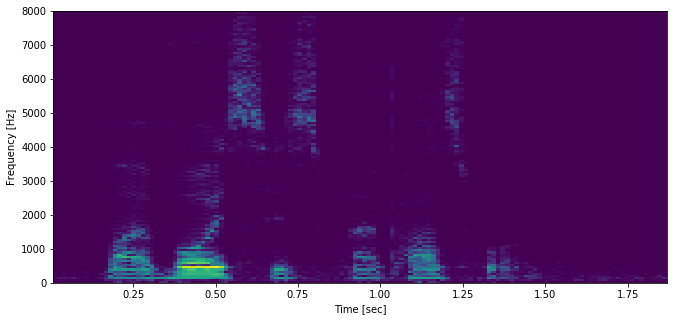
\includegraphics[width=0.8\textwidth]{images/2_1_a_example_spectrogram}
    \caption{Spektrogram sygnału \code{m0002/20150713085938321\underscore m0002\underscore 31.pcm} ze zbioru RedDots}
    \label{fig:2_1_a_example_spectrogram}
\end{figure}

\begin{figure}[H]
    \centering
    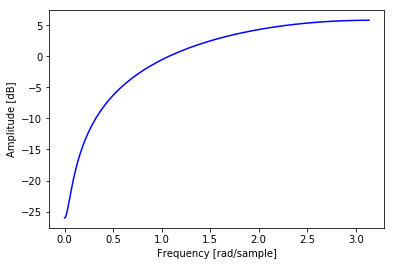
\includegraphics[width=0.6\textwidth]{images/2_1_c_preemphasis_response}
    \caption{Odpowiedź impulsowa \foreign{preemphasis} $[-0.95, 1.0]$}
    \label{fig:2_1_c_preemphasis_response}
\end{figure}

\begin{figure}[H]
    \centering
    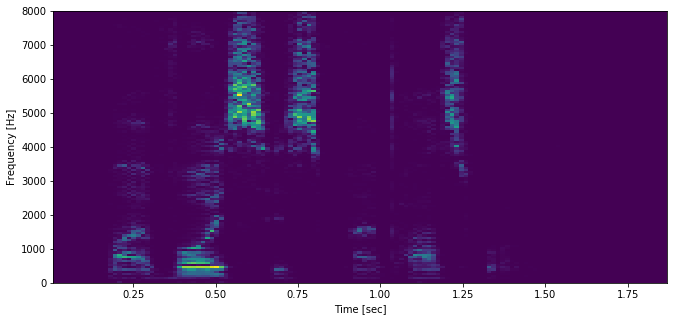
\includegraphics[width=0.8\textwidth]{images/2_1_b_example_preemphasis}
    \caption{Spektrogram tego samego sygnału poddany \foreign{preemphasis}}
    \label{fig:2_1_b_example_preemphasis}
\end{figure}

Jak pokazuje \ref{fig:2_1_b_example_preemphasis}, energia w wyższych pasmach po tej operacji
została wyrównana z energią w niższych pasmach częstotliwości. Ogranicza to błędy numeryczne
pojawiające się przy dalszym przetwarzaniu, co miało duże znaczenie w starszych komputerach.

W drugim kroku należy policzyć \foreign{Short Time Fourier Transform}, to znaczy podzielić
sygnał na ramki i dla każdej ramki policzyć spektrum częstotliwościowe. Typowa szerokość
okna to $25$ms, przy czym każde kolejne okno jest przesunięte o ok. połowę szerokości, 
np. można przyjąć $10$ms. W przypadku zbioru RedDots nagrania mają częstotliwość próbkowania $16$kHz,
więc by uzyskać takie przesunięcie okna muszą zawierać $400$ próbek z przesunięciem $160$ próbek.
Następnie spektra zamieniane są w spektra mocy przez wzięcie kwadratu wartości absolutnej
z każdej wartości w spektrum.

Wynik \shortcut{STFT} można zwizualizować jako spektrogram, jak na \ref{fig:2_1_a_example_spectrogram}, 
i zawiera on informacje o tym jak energia sygnału w różnych pasmach zmieniała się w czasie. 
Każde okno można wyciąć z użyciem okna Hamminga lub Hanna, które mają mniejszy wpływ
na wynikowe spektrum sygnału niż okno prostokątne. (Wycięcie wybranego przedziału próbek
z sygnału jest równoważne przemnożeniu przez okno prostokątne)

Następnie budowany jest bank filtrów w skali Mela. Przeliczenia częstotliwości Melach na
częstotliwość w Hertzach dokonuje się według poniższych wzorów. 

$$m = 2595 log_{10}(1 + \frac{f}{700})$$
$$f = 700 (10^{m/2595} - 1)$$

Jest to skala w nieliniowej zależności z Hertzami. Jej postać i stałe zostały tak dobrane,
że zmiana w tej skali odpowiada subiektywnemu odczuciu zmiany wysokości dźwięku przez ludzi.

Bank filtrów składa się z pewnej liczby, zwykle $20$ lub $26$, trójkątnych filtrów o równej
szerokości w skali Mela, rozmieszczonych z przesunięciem 50\% szerokości. Ich szerokość
jest tak dobrana, by pokryły cały przedział częstotliwości sygnału.

\begin{figure}[H]
    \centering
    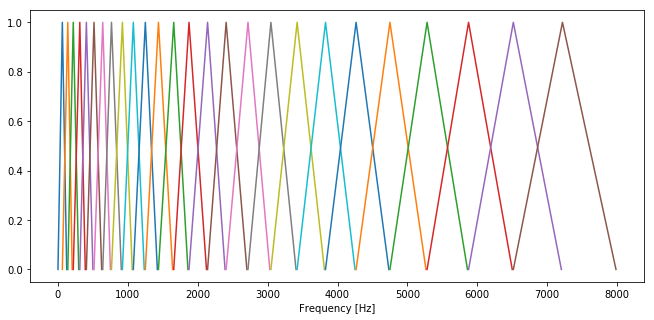
\includegraphics[width=0.8\textwidth]{images/2_1_d_mel_filters}
    \caption{Charakterystyka w skali Hertza banku 20 trójkątnych filtrów o równej szerokości w skali Mela}
    \label{fig:2_1_d_mel_filters}
\end{figure}

Mając te filtry następnym etapem przetwarzania sygnału jest przemnożenie przez każdy z tych filtrów i zsumowanie 
dzięki czemu uzyskuje się jedną liczbę na filtr - całkowitą energię sygnału na pokrytych filtrami pasmach.

Sumy są następnie logarytmowane. Pozwala to na dekonwolucję sygnału mowy i wpływu środowiska. 
Dekonwolucja przebiega w ten sposób, że najpierw dzięki policzeniu transformaty Fouriera,
uzyskiwane jest spektrum, a konwolucja sygnału w czasie jest równoważna przemnożeniu widm częstotliwościowych.
Następnie jak ten iloczyn widm zostanie zlogarytmowany, to oba można go przedstawić jako sumę logarytmów.
W wynikowych cechach jeżeli sygnał mowy został z czymś spleciony, to skutkuje to tylko przesunięciem cech
ze wszystkich ramek. Można wtedy, przy założeniu, że wpływ otoczenia jest stały, znormalizować średnią tych cech, 
by zmniejszyć jego wpływ. 

Znormalizowane współczynniki filtrów Mela bywają używane jako gotowy zestaw cech. Do uzyskania \shortcut{MFCC}
potrzebne jest jeszcze policzenie dyskretnej transformaty cosinusowej. Dyskretna transformata cosinusowa to modyfikacja
transformaty Fouriera, która w wyniku daje ciąg współczynników rzeczywistych, a nie zespolonych. Wykorzystana jest
właściwość \shortcut{DFT}, że jeżeli sygnał w dziedzinie czasu ma współczynniki rzeczywiste, to współczynniki transformaty
będą Hermitian-symetryczne. A jeżeli sygnał w dziedzinie czasu jest symetryczny, to transformata będzie miała
tylko współczynniki rzeczywiste. \shortcut{DCT} liczy się zatem tak, iż tworzony jest nowy sygnał dwa razy większej długości niż
sygnał wyjściowy, przez odbicie wyjściowego sygnału. Taki sygnał będzie symetryczny i rzeczywisty, więc jego transformata
Fouriera będzie również symetryczna i rzeczywista. Połowę transformaty można odrzucić, a druga połowa, zawierająca
współczynniki rzeczywiste i będąca takiego samego rozmiaru co wyjściowy sygnał, nazywamy dyskretną transformatą cosinusową.

Fakt, że \shortcut{DCT} sygnału jest również rzeczywista i ma ten sam rozmiar jest wygodny, lecz liczy się ją, 
gdyż ma właściwości dekorelacyjne. Dzięki temu przy modelowaniu \shortcut{MFCC} za pomocą wielowymiarowej 
dystrybucji normalnej można przyjąć, że
współczynniki są nieskorelowane i zastosować uproszczenie, że macierz kowariancji parametryzująca tę dystrybucję 
jest macierzą diagonalną.

\begin{figure}[H]
    \centering
    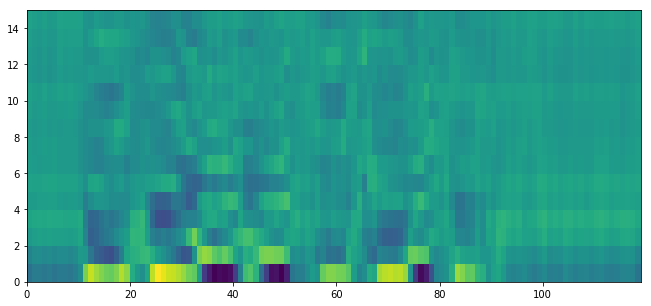
\includegraphics[width=0.8\textwidth]{images/2_1_e_mfcc}
    \caption{Wizualizacja 15 pierwszych współczynników \shortcut{MFCC} dla każdej ramki przykładowego sygnału}
    \label{fig:2_1_e_mfcc}
\end{figure}

Wynik \shortcut{DCT} nazywamy \foreign{Mel-frequency cepstral coefficients} i ze względu na wspomniane właściwości użyjemy ich
w naszych systemach. W praktyce z $26$ współczynników wybiera się tylko pierwsze $13$ lub $20$, gdyż dalsze opisują
wysokie częstotliwości, które są nieprzydatne przy rozumieniu sygnału mowy. Do tych współczynników dołącza się $26$ lub $40$
współczynników delta oraz delta-delta. Współczynniki delta mają opisać jak konkretne współczynniki zmieniają się w czasie,
choć zapewne tracą na przydatności w modelach jak sieci neuronowe, które mogą na wejściu przyjąć nie tylko jedną ramkę sygnału,
ale też kilka sąsiadujących ramek. 

\begin{figure}[H]
    \centering
    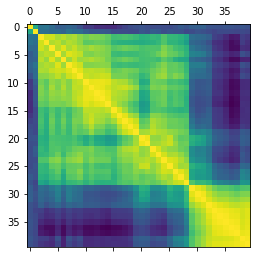
\includegraphics[width=0.6\textwidth]{images/2_1_f_correlation_matrix_banks}
    \caption{Macierz korelacji dla współczynników uzyskanych z banku filtrów}
    \label{fig:2_1_f_correlation_matrix_banks}
\end{figure}

\begin{figure}[H]
    \centering
    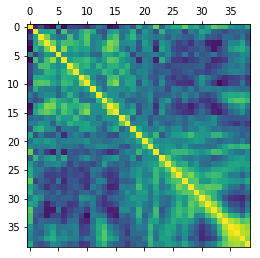
\includegraphics[width=0.6\textwidth]{images/2_1_g_correlation_matrix_mfcc}
    \caption{Macierz korelacji dla współczynników \shortcut{MFCC}}
    \label{fig:2_1_g_correlation_matrix_mfcc}
\end{figure}

\subsection{Mikstury gaussowskie}\label{sec:gmm}

Mikstura rozkładów to sposób opisu rozkładu zmiennej losowej $X$ przez wprowadzenie dodatkowej ukrytej zmiennej $\Theta$.
Następnie uznaje się, że dla każdej wartości zmiennej ukrytej rozkład zmiennej pochodzi z innego rozkładu.
Zwykle zmienna ukryta jest dyskretna, wyjściowa zmienna może być dyskretna lub ciągła i przyjmuje się, że wszystkie
warunkowe rozkłady $P(X|\Theta)$ pochodzą z tej samej rodziny i różnią się parametrami. Rozkład zmiennej $X$ można
uzyskać przez marginalizację zmiennej ukrytej.

$$f(x) = \sum_{\theta_i} f(X | \theta_i) P(\theta_i)$$

Przy miksturach gaussowskie przyjmuje się, że warunkowe prawdopodobieństwa zmiennej wyjściowej od zmiennej ukrytej
należą do rodziny wielowymiarowych rozkładów normalnych, tj. mają gęstość

$$f(x | \theta_i) = \frac{1}{\sqrt{(2 \pi)^d |\Sigma_i|}} exp(-\frac{1}{2} (x - \mu_i)^T \Sigma_i^{-1} (x - \mu_i))$$

gdzie $\mu_i$ to $d$ wymiarowy wektor średnich, $\Sigma_i$ to macierz kowariancji rozmiaru $d \times d$

\subsection{Maksymalizowanie wartości oczekiwanej}\label{sec:gmm}

Parametry wielowymiarowego rozkładu normalnego można wyestymować na podstawie próby, na przykład 
stosując estymator maksymalizujący prawdopodobieństwo danych.

Estymatory parametrów maksymalizujące prawdopodobieństwo $M$ elementów $x^j$.

$\hat{\mu} = \frac{1}{m} \Sigma_{j=0}^M x^{j}$

$\hat{\Sigma} = \frac{1}{m} \Sigma_{j=0}^M (x^{j} - \hat{\mu})^T (x^{j} - \hat{\mu})$

Jednak w przypadku mikstury, jeżeli nie przypiszemy z góry próbek wybranym wartościom ukrytej zmiennej, problem 
estymacji parametrów wymaga innego podejścia. Jedną z metod jest \foreign{Expectation Maximization}, iteracyjny 
algorytm wyznaczania wartości parametrów dla mikstur dystrybucji lub ogólniej dla modeli z ukrytymi zmiennymi. 
Składa się z dwóch kroków wykonywanych na zmianę do zbieżności:

\begin{itemize}
    \item \foreign{Expectation} -  % todo
    \item \foreign{Maximization} - 
\end{itemize}

Algorytm nie gwarantuje znalezienia globalnie optymalnego rozwiązania.

\subsection{Dynamic Time Warping}\label{sec:dtw}

Jako że praca dotyczy rozpoznawania zależnego od tekstu, konieczne by uzyskać wartościowe wyniki będzie
użycie metod pozwalających na uwzględnienie informacji o sekwencji ramek. Samo dopasowanie mikstur do ramek
tej informacji nie uwzględni. Jedną z takich metod jest \foreign{dynamic time warping}.

\shortcut{DTW} to algorytm do porównywania dwóch ciągów. Ciągi mogą być różnej długości i algorytm zwróci
dla nich wysokie podobieństwo (małą odległość) nawet jeśli pewne podciągi będą bardziej rozciągnięte lub krótsze 
w jednym ciągu niż w drugim. 

Algorytm wymaga wybrania metryki (oznaczmy ją $d$) określającą odległość pojedynczych elementów ciągu.

\shortcut{DTW} wykorzystuje technikę programowania dynamicznego i w podstawowej wersji znanej autorowi wymaga liczby operacji 
rzędu $\Theta(n \times m)$, gdzie $n$ i $m$ to długości porównywanych ciągów oraz ma złożoność pamięciową liniową
względem długości krótszego ciągu. Istnieją jego bardziej wydaje wersje, w tym wersje z oknem, tzn. bazujące na 
założeniu, że nie ma sensu porównywać elementów z dwóch ciągów ze zbyt odległymi indeksami.

Algorytm wygląda tak: Na początku inicjalizowana jest macierz odległości $D$ rozmiaru $n + 1 \times m + 1$. Pierwszy
rząd i pierwsza kolumna jest wypełniana cyfrową reprezentacją $\infty$, co oznacza tyle, 
że te wartości nie są brane pod uwagę w następnym kroku.
Wyjątkiem jest komórka w pierwszym rzędzie i pierwszej kolumnie z wartością $D_{0,0} = 0$.

Pozostałe wartości macierzy są liczone ze wzoru

$$D_{i+1, j+1} = min(D_{i+1, j}, D_{i, j+1}, D_{i, j}) + d(N_i, M_j)$$

gdzie $N_i$ i$M_j$ oznaczają elementy porównywanych ciągów, a $d(N_i, M_j)$ to jak już wspomniano wybrana 
niezależnie od algorytmu odległość między dwoma elementami. Odległość ciągów od siebie znaleziona przez \shortcut{DTW}
to $D_{n, m}$.  Licząc te wartości rzędami możliwe jest osiągnięcie liniowej złożoności pamięciowej względem
długości krótszego ciągu.

Powyższy wzór na $D_{i+1, j+1}$ należy zinterpretować tak, że liczymy odległość pary elementów $N_i$, $M_j$ i dodajemy
do najbardziej korzystnego wyniku z pośród trzech opcji:

\begin{itemize}
    \item Wybór $D_{i+1, j}$ oznacza, że obecny rezultat składa się z $d(N_i, M_{j-1})$ i $d(N_i, M_j)$, a więc ten sam element ciągu $N$ jest porównany z dwoma elementami ciągu $M$. Na przykład w $N = [1, 20, 20, 20, 20]$, $M = [1, 1, 1, 10]$ i odległości różnicy absolutnej ten przypadek będzie kilka razy najkorzystniejszy.
    \item Wybór $D_{i, j+1}$ oznacza, że w sumie będzie zarazem $d(N_{i-1}, M_j)$ i $d(N_i, M_j)$, a więc dwa elementy ciągu $N$ są porównane z tym samym elementem ciągu $M$. Na przykład w wyniku dla $N = [1, 1, 1, 1, 1, 20]$ i $ M = [1, 10]$ ten przypadek będzie się składał na wynik minimalizujący odległość ciągów.
    \item $D_{i, j}$ oznacza, że obliczono odległość następnego elementu zarówno z ciągu $N$ i z ciągu $M$. Przy porównywaniu $N = [1, 2, 3, 4]$ oraz $M = [1, 2, 3, 4]$ zajdzie wyłącznie on.
\end{itemize}

Poniżej przedstawiono kilka przykładów tabelek z wynikami $DTW$. Elementami są liczby, a w roli metryki jest kwadrat różnicy.

\begin{table}[H]
    \caption{Macierz $D$ dla $DTW$ na dwóch przykładowych sekwencjach $N$ i $M$. Przykład gdy elementy jednej sekwencja są wielokrotnie dopasowana do pierwszego elementu z drugiej sekwencji, dopóki jest to możliwe.}
    \centering
    \label{tab:dtw_example0}
    \small
    \tabulinesep =_3pt^3pt
    \begin{tabu}{r*{7}{r}}
        \multirow{2}{*}{} & & \multicolumn{5}{c}{N}
        \\
        & & - & 1 & 20 & 20 & 20 & 20
        \\ \midrule
        \multirow{5}{*}{M} & - & 0 & $\infty$ & $\infty$ & $\infty$ & $\infty$ & $\infty$
        \\ 
        & 1 & $\infty$ & 0 & 19 & 38 & 57 & 76
        \\
        & 1 & $\infty$ & 0 & 19 & 38 & 57 & 76
        \\
        & 1 & $\infty$ & 0 & 19 & 38 & 57 & 76
        \\
        & 10 & $\infty$ & 9 & 10 & 20 & 30 & \textbf{40}
        \\
    \end{tabu}
\end{table}

\begin{table}[H]
    \caption{Macierz $D$ dla $DTW$ na dwóch przykładowych sekwencjach $N$ i $M$. Przykład z dokładnie dopasowanymi sekwencjami, z wydłużonymi lub skróconymi fragmentami.}
    \centering
    \label{tab:dtw_example1}
    \small
    \tabulinesep =_3pt^3pt
    \begin{tabu}{r*{11}{r}}
        \multirow{2}{*}{} & & \multicolumn{9}{c}{N}
        \\
        & & - & 1 & 1 & 2 & 3 & 3 & 3 & 4 & 4
        \\ \midrule
        \multirow{7}{*}{M} & - & 0 & $\infty$ & $\infty$ & $\infty$ & $\infty$ & $\infty$ & $\infty$ & $\infty$ & $\infty$
        \\
        & 1 & $\infty$ & 0 & 0 & 1 & 3 & 5 & 7 & 10 & 13
        \\
        & 2 & $\infty$ & 1 & 1 & 0 & 1 & 2 & 3 & 5 & 7
        \\
        & 2 & $\infty$ & 2 & 2 & 0 & 1 & 2 & 3 & 5 & 7
        \\
        & 2 & $\infty$ & 3 & 3 & 0 & 1 & 2 & 3 & 5 & 7
        \\
        & 3 & $\infty$ & 5 & 5 & 1 & 0 & 0 & 0 & 1 & 2
        \\
        & 4 & $\infty$ & 8 & 8 & 3 & 1 & 1 & 1 & 0 & \textbf{0}
        \\
    \end{tabu}
\end{table}

\subsection{Ukryte modele Markowa}\label{sec:hmm}

Ukryty model Markowa to proces stochastyczny, dyskretny w czasie, pozwalający na modelowanie dystrybucji 
sekwencji zdarzeń. Będzie zatem użyteczny ze względu na możliwość uwzględnienia w nim zależności 
między ramkami w czasie.

Model składa się z zbioru $N$ ukrytych stanów $X = \{x_0, x_1, \dots\, x_{N-1}\}$, ciągu zmiennych losowych
$X_t$, $t = 0, 1, \dots, T - 1$ oznaczających ukryty stan w chwili $t$, rozkładu początkowego stanu ukrytego
$\pi_i = P(X_0 = x_i)$, zbioru obserwacji (emisji, stan jawny) $Y$, przy czym obserwacje mogą być dyskretne 
lub ciągłe i ciągu zmiennych losowych $Y_t$, $t = 0, 1, \dots, T - 1$ określających obserwację w chwili $t$.

Do tego zdefiniowane są prawdopodobieństwa przejść między stanami oraz rozkłady obserwacji w każdym stanie. 
Kluczową kwestią w modelu Markowa, zwaną regułą Markowa, jest iż rozkład prawdopodobieństwo następnego stanu $X_t$ 
zależy wyłącznie od stanu poprzedzającego, nie jest ważna cała historia stanów w przeszłości. Podobnie rozkład
obserwacji $Y_t$ zależy wyłącznie od obecnego stanu ukrytego. 

Inną właściwością, którą się przyjmuje, jest jednorodność. Oznacza to, że przejścia między stanami i emisje są
niezależne od czasu $t$. Przy dyskretnych i jednorodnych stanach ukrytych prawdopodobieństwa przejść
między stanami można zapisać w postaci macierzy $H$ (\foreign{transition matrix}) $P(X_t = x_i | X_{t-1} = x_j) = H_{j, i}$.
Podobnie jeżeli emisje są dyskretne, to można je zapisać w postaci macierzy $V$ $P(Y_t = y_i | X_t = x_j) = V_{j, i}$.
Lecz emisje często mają jakieś określone parametryczne dystrybucje i wtedy definiuje się w postaci wektorów parametrów.

Czasami, w innych modelach regułę Markowa rozszerza się tak, iż prawdopodobieństwo może zależeć od $k$ ostatnich stanów
$P(X_t | X_{t-1} \dots X_{t-k}$ i nazywa się to regułą Markowa $k$ rzędu. Są też inne wersje, w których zbiór
ukrytych stanów jest ciągły, w których rząd $k$ jest funkcją czegoś lub na przykład pola Markowa, 
gdzie nie mówimy o ciągu w czasie, lecz o zmiennych rozmieszczonych
w kilku wymiarach, których wartości zależą od najbliższego otoczenia. Wszystkie modele Markowa mają jednak cechę wspólną, iż
zmienne losowe zależą w nich od pewnego skończonego otoczenia.

Jeżeli macierz przejść jest tak zdefiniowana, że zawsze możliwe jest przejście z każdego stanu do każdego, to
mówimy, że model jest ergodyczny. Jednak na przykład w rozpoznawaniu mowy często definiuje się macierz przejść,
by pozwalała tylko na przejście do stanu o takim samym lub wyższym indeksie, tzw. model Bakisa lub model lewo-prawo 
(\foreign{left-to-right}) albo by pozwalała wyłącznie na przejście z danego stanu do tego samego stanu lub stanu
o indeksie o jeden większym. (model \foreign{beads-on-string})

Ważne w praktyce jest, że istnieją wydajne algorytmy rozwiązujące następujące problemy \shortcut{HMM}:

\begin{enumerate}
    \item Algorytm w przód - problem znalezienia prawdopodobieństwa stanu ukrytego w danej chwili wraz z pewnym ciągiem obserwacji do tego chwili. Jeżeli tym punktem w czasie będzie koniec sekwencji obserwacji, to można zmarginalizować prawdopodobieństwo końcowego stanu i uzyskać prawdopodobieństwo wygenerowania danej sekwencji obserwacji przez model.
    \item Algorytm w tył - problem znalezienia prawdopodobieństwa stanu ukrytego w danej chwili pod warunkiem wystąpienia danego ciągu zdarzeń w przyszłości. Interpretacja może być nieintuicyjna, lecz jest on istotny, gdyż jest częścią następnego algorytmu.
    \item Algorytm w przód i w tył - problem znalezienia prawdopodobieństwa stanu ukrytego w danej chwili pod warunkiem wystąpienia danego ciągu obserwacji. Brany pod uwagę jest cały ciąg obserwacji, tych przed i tych po danym stanie ukrytym. Działa przez połączenie wyników algorytmu w przód i w tył, stąd nazwa. 
    \item Algorytm Viterbiego - problem znalezienia najbardziej prawdopodobnego ciągu stanów ukrytych dla danego ciągu obserwacji parametrów modelu. Jest podobny do algorytmu w przód, z tym, że na każdym kroku wybiera najbardziej prawdopodobną sekwencję zamiast uwzględniać prawdopodobieństwa wszystkich stanów.
    \item Algorytm Bauma-Welcha - problem znalezienia parametrów modelu Markowa (prawdopodobieństwo przejść między stanami ukrytymi, rozkład obserwacji dla każdego stanu ukrytego, rozkład stanu początkowego) maksymalizującego prawdopodobieństwo wystąpienia danego ciągu obserwacji. Wykorzystuje algorytm w przód i w tył oraz opisany wcześniej algorytm \foreign{expectation maximization}, algorytm \foreign{forward-backward} służy do wyznaczenia ukrytych zmiennych opisujących jaki był stan w każdej chwili czasu na potrzeby kroku \foreign{expectation}, a następnie wyznaczane są najbardziej prawdopodobne parametry emisji w kroku \foreign{maximization}.
\end{enumerate}

\subsubsection{Algorytm w przód}
\foreign{Forward algorithm}

\subsubsection{Algorytm w tył}
\foreign{Backward algorithm}

\subsubsection{Algorytm w przód i w tył}
\foreign{Forward-Backward algorithm}

\subsubsection{Algorytm Viterbiego}
\foreign{Viterbi algorithm}

\subsubsection{Algorytm Bauma-Welcha}
\foreign{Baum-Welch algorithm}

% cite Rabiner Tutorial

\section{Rozpoznawanie mówcy}\label{sec:rozpoznawanie_mowcy}

% train / enroll / test

% MAP adaptacja

% LDA ?

% ROC, EER, AUC

\section{Istniejące systemy weryfikacji mówcy}\label{sec:istniejace_systemy}

% GMM UBM
% i-vectors
% DTW
% HMM GMM
% HMM DNN
% Bottleneck
% googlowe g-vectors (to było ich?)
